\documentclass[11pt]{article}
\usepackage[margin=1in]{geometry}
\usepackage{booktabs}
\usepackage{graphicx}
\usepackage{amsmath,amssymb}
\usepackage{hyperref}

\title{Beyond Oracle Knowledge Editing: Blind Discovery and Evidence-Gated Repair of Corrupted Knowledge in Language Models}
\author{Anonymous Authors (Draft for Human Author Review)}
\date{November 2026}

\begin{document}
\maketitle

\begin{abstract}
Existing knowledge editing methods assume an oracle edit request specifying both which factual association is corrupted and what the target ground-truth answer should be. We study \emph{Selective Knowledge Repair under Uncertainty}: given only a corrupted language model $M_d$, a public knowledge pool $U$ without ground-truth answers, general relational rules $R$, and explicit query/write budgets $(B_q, B_w)$, can a blind repair pipeline discover degraded facts, assess whether residual internal semantics suffice to reconstruct a reliable candidate, and safely persist weight updates without damaging healthy or immutable same-entity knowledge? Across brand-new entity pools disjoint from prior development sets (50 new entities in v0.6; 52 in v0.5) and two 3B model families (\texttt{Qwen2.5-Omni-3B} and \texttt{Llama-3.2-3B-Instruct}), we establish three empirical findings: (1) Under equal-budget blind discovery, reversed-entropy detects overconfident wrong-fact injections at minimal cost ($\text{AUPRC}=0.676$ at 50 queries) but misses $100\%$ of uninjected collateral degradations ($0/7$), whereas constraint-discrepancy detection achieves the highest AUROC ($0.724$), lowest healthy FPR ($0.143$), and $71.4\%$ collateral recall. (2) Structured evidence reconstruction outperforms generative reconstruction ($73.7\%$ vs.\ $21.1\%$, $+52.6$~pp) and passes $100\%$ of sham-invariance, hitting-set abstention, and twin-world unidentifiability controls, though within already-covered structured candidates heuristic support scores do not beat simple confidence on AURC. (3) Crucially, in true sequential multi-target end-to-end repair ($8$ cumulative \texttt{standard\_kl} LoRA merges audited via isolated fresh subprocesses), while evidence-gated repair triples raw recovery over generative baselines ($6/19$--$8/19$ vs.\ $2/19$) with $0$ known wrong writes and cuts same-entity regressions by $31\%$--$38\%$, \emph{every} strategy---including gold Oracle ($3$ regressions masked by $11$ improvements)---violates strict per-fact same-entity zero-regression locality ($Y=0.0$) despite $0.0\%$ general commonsense drop. We release our isolated audit protocol, negative results, and fresh-subprocess verification harness to ground future work on safe sequential blind repair.
\end{abstract}

\section{Introduction}
Classical parametric knowledge editing methods such as ROME~\cite{meng2022rome}, MEMIT~\cite{meng2023memit}, and AlphaEdit~\cite{fang2025alphaedit} assume two strong oracles: (i) the identity of the corrupted fact is given, and (ii) the desired ground-truth target answer is provided. In deployed models affected by accidental mis-fine-tuning or localized corruption, neither oracle is available. We formalize \emph{Blind Knowledge Repair} under strict public/evaluator information isolation and evaluate whether residual semantic relations inside the damaged model enable safe, persistent restoration without hiding failure modes.

\section{Related Work}
Our work sits at the intersection of parametric knowledge editing~\cite{meng2022rome,meng2023memit,fang2025alphaedit}, ripple and locality evaluation~\cite{cohen2024rippleedits}, budgeted deficiency discovery (SEA~\cite{sea2025colm}), edit detection (\emph{Has this Fact been Edited?}~\cite{editdetect2025naacl}), residual associative leakage (ThinkEval~\cite{thinkeval2026tmlr}), and recent self-rewriting studies~\cite{selfrewrite2026arxiv}. Unlike ThinkEval (which diagnoses residual leakage) or SEA (which queries an external knowledge base), we study internal-only blind discovery, support-structure gating, and cumulative sequential LoRA persistence under per-fact locality auditing.

\section{Problem Definition and Information Boundaries}
Let $u = (\text{entity}, \text{relation}, \text{access\_path})$ be a public knowledge unit containing no ground-truth label. Given a multi-target damaged model $M_d$, a shuffled public pool $U$, domain-general relational rules $R$, query budget $B_q$, and write budget $B_w$, a blind repair method outputs a sequence of actions in $\{\text{ATTEMPT\_REPAIR}, \text{ABSTAIN}, \text{REQUEST\_EVIDENCE}\}$. Evaluator-only artifacts (clean weights, gold answers, planned damage list, hidden locality controls) are strictly isolated from non-Oracle methods. Our primary endpoint is \emph{End-to-End Strict Safe Repair Yield} ($Y$): the fraction of all paired-degraded units $D$ (planned plus collateral) restored on held-out probes in a fresh subprocess that simultaneously satisfies per-fact zero-regression same-entity locality and group retention gates ($Y=\text{NA}$ if $D=0$).

\section{Method}
Our pipeline consists of three modular stages: (1) budgeted blind discovery combining direct-probe stability and atomic-fact constraint conflict, (2) 8-class support-structure analysis over minimal support sets $C(E, R)$ distinguishing \texttt{single\_decisive}, \texttt{redundant\_distinct\_attributes} (explicitly intra-model, never external independent sources), \texttt{single\_chain}, \texttt{redundant\_same\_source}, \texttt{conflicting\_support}, and \texttt{insufficient\_support}, and (3) sequential \texttt{standard\_kl} LoRA writeback ($r=8$, $\alpha=16$, last 4 layers, 32 steps, KL retain weight $50.0$) guarded by unlabeled public retain self-checks and rollback.

\section{Evaluation Protocol}
We evaluate on a frozen, shuffled 50-entity v0.6 pilot pool ($36$ verifiable real facts + $6$ obscure real unknowns + $4$ fictional unknowns + $4$ ambiguous controls, verified $0$ normalized-name/alias overlap with all $192$ historical v0.3/v0.5 entities; SHA256 \texttt{95b845901b2f}). Ground truth is defined by paired pre/post held-out accuracy ($\text{clean}=1.0$, $\text{post}\le 0.5$, $\Delta \ge 0.5$). Every final sequential model $M_f$ is reconstructed from base weights, `damaged\_state.pt` (SHA256-checked), and all committed adapters in an isolated fresh Python subprocess.

\section{Results}
\subsection{Equal-Budget Blind Discovery (G1)}
\begin{table}[t]
\centering\small
\caption{Equal-budget blind discovery on the 50-entity v0.6 pool (\texttt{Qwen2.5-Omni-3B}, $D=19$: 12 planned D1 + 7 collateral, budget cap $5N=250$).}
\begin{tabular}{lrrrrrrr}
\toprule
Detector & LogQ & Tok & AUPRC & AUROC & P@25\% & H-FPR & ColRec \\
\midrule
low\_confidence & 50 & 3069 & 0.363 & 0.362 & 0.417 & 0.286 & 0.429 \\
high\_confidence\_rev & 50 & 3069 & 0.672 & 0.638 & 0.667 & 0.429 & 0.000 \\
entropy & 50 & 3069 & 0.340 & 0.353 & 0.500 & 0.357 & 0.857 \\
neg\_entropy\_rev & 50 & 3069 & 0.676 & 0.647 & 0.667 & 0.357 & 0.000 \\
self\_consistency & 100 & 6106 & 0.312 & 0.324 & 0.167 & 0.286 & 0.286 \\
repeated\_paraphrases\_perm & 250 & 15363 & 0.420 & 0.591 & 0.333 & 0.714 & 1.000 \\
direct\_vs\_constraint & 201 & 8797 & 0.626 & 0.724 & 0.500 & 0.143 & 0.714 \\
m2\_reference\_free & 250 & 11871 & 0.479 & 0.650 & 0.500 & 0.143 & 0.714 \\
full\_m2 & 250 & 11871 & 0.479 & 0.650 & 0.500 & 0.429 & 0.857 \\
\bottomrule
\end{tabular}
\end{table}

\begin{figure}[t]
  \centering
  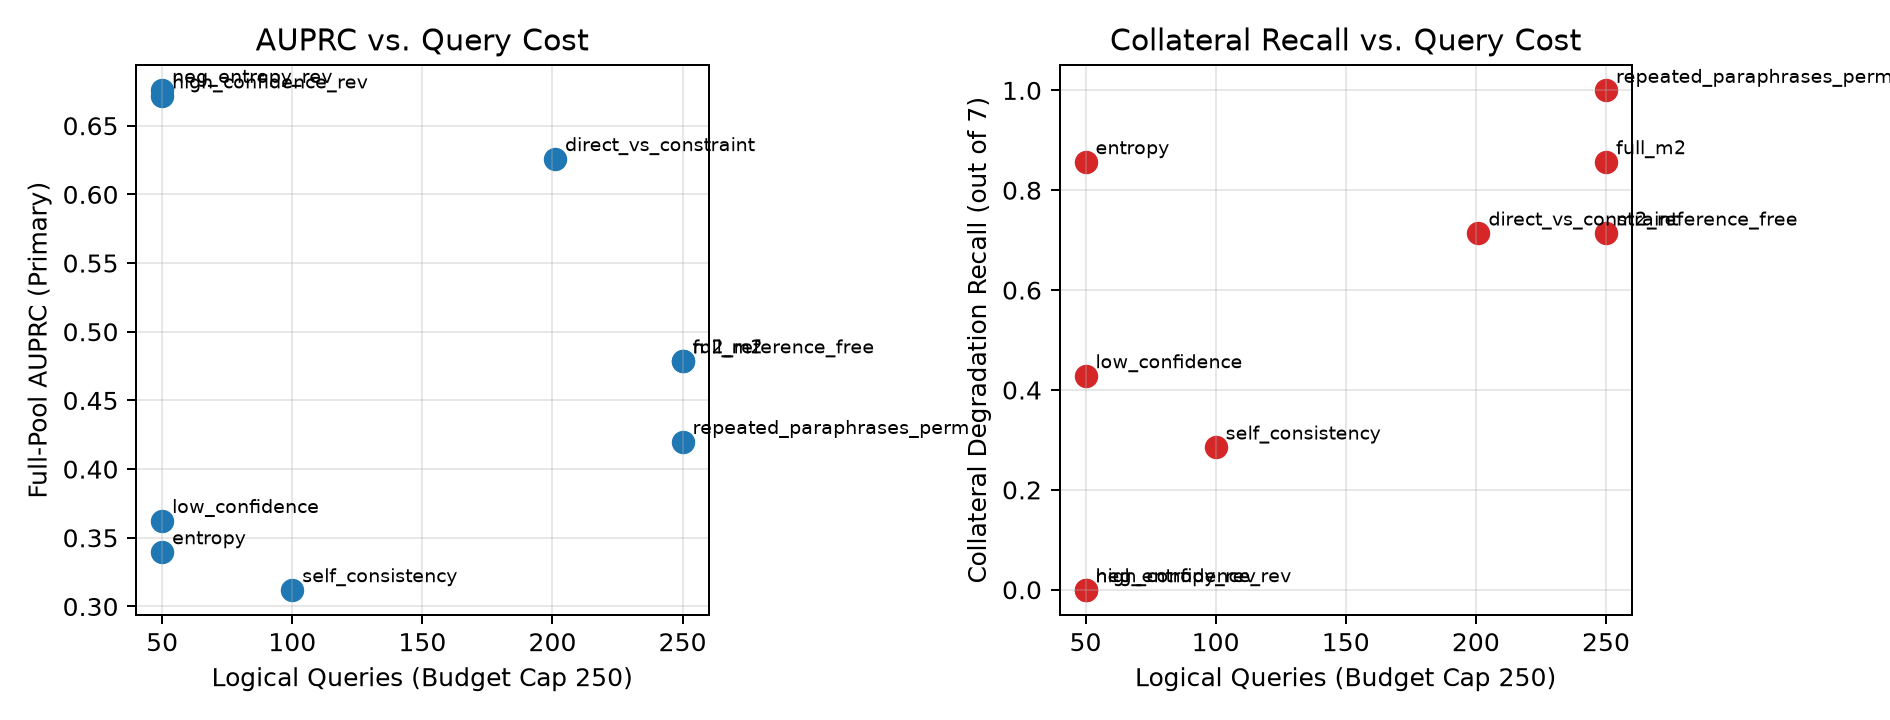
\includegraphics[width=0.88\linewidth]{figures/fig2_detection_cost.png}
  \caption{Full-pool AUPRC and collateral recall vs.\ logical query cost on the 50-entity v0.6 pool ($D=19$: 12 planned D1 + 7 collateral). Reversed entropy excels at planned overconfident D1 but misses all 7 collateral degradations ($0/7$), while \texttt{direct\_vs\_constraint} achieves the highest AUROC ($0.724$) and $71.4\%$ collateral recall.}
\end{figure}

\subsection{True End-to-End Sequential Blind Repair (G1 E2E)}
\begin{table}[t]
\centering\small
\caption{True sequential multi-target E2E blind repair on \texttt{Qwen2.5-Omni-3B} ($D=19$, $B_w=8$, isolated fresh-subprocess reload audit).}
\begin{tabular}{lrrrrrrr}
\toprule
Strategy & Comm & Raw Rest. & Active & WW & UnkAtt & SE-Reg & Strict $Y$ \\
\midrule
B0\_no\_repair & 0 & 0/19 & 0 & 0 & 0 & 0 & 0.00 \\
B1\_generative & 8 & 2/19 & 1 & 0 & 4 & 16 & 0.00 \\
B2\_ungated\_structured & 8 & 7/19 & 3 & 0 & 3 & 12 & 0.00 \\
B3\_confidence\_gate & 8 & 2/19 & 0 & 0 & 4 & 17 & 0.00 \\
B3\_fact\_count\_gate & 8 & 6/19 & 4 & 0 & 3 & 10 & 0.00 \\
B3\_random\_gate & 8 & 6/19 & 4 & 1 & 3 & 9 & 0.00 \\
M\_evidence\_gated & 8 & 6/19 & 4 & 0 & 3 & 11 & 0.00 \\
M\_full & 8 & 8/19 & 5 & 0 & 2 & 10 & 0.00 \\
Oracle\_upper\_bound & 8 & 19/19 & 8 & 0 & 0 & 3 & 0.00 \\
\bottomrule
\end{tabular}
\end{table}

Crucially, even \texttt{Oracle\_upper\_bound} ($19/19$ raw recovery, $0$ harmed healthy, $0.000$ general commonsense drop) incurs $3$ same-entity regressions across $8$ cumulative LoRA merges (masked by $11$ wrong-to-correct shifts in group mean accuracy), yielding strict $Y=0.0$ across all strategies.

\subsection{Fixed-Candidate Risk--Coverage and Full-Policy Interventions (G2-A)}
\begin{figure}[t]
  \centering
  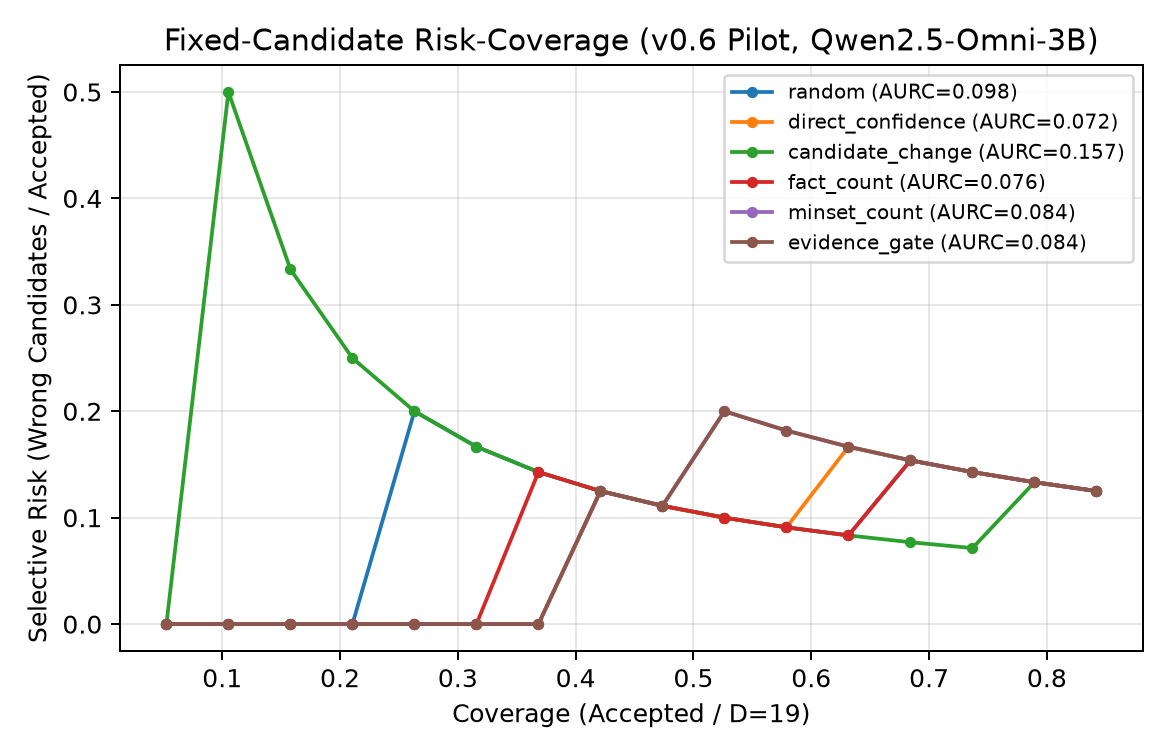
\includegraphics[width=0.85\linewidth]{figures/fig3_risk_coverage.png}
  \caption{Fixed-candidate risk--coverage curves over the $D=19$ degraded targets ($16/19$ covered by structured reconstruction, $14/16$ correct).}
\end{figure}
Structured reconstruction outperforms generative reconstruction ($73.7\%$ vs.\ $21.1\%$, $+52.6$~pp). Full-policy interventions achieve $100\%$ sham invariance ($19/19$), $100\%$ hitting-set abstention ($15/15$), $94.7\%$ counterfactual sensitivity ($18/19$), $0\%$ correlated-duplicate fooling ($0/19$), and $100\%$ twin-world abstention ($2/2$). Within already-covered structured candidates, heuristic support scores ($\text{AURC}=0.084$) do not beat direct confidence ($0.072$) or fact count ($0.076$).

\subsection{Cross-Architecture Persistence (\texttt{Llama-3.2-3B-Instruct})}
\begin{table}[t]
\centering\small
\caption{Cross-architecture true sequential E2E persistence on \texttt{Llama-3.2-3B-Instruct} (isolated fresh-subprocess reload).}
\begin{tabular}{lrrrrrrr}
\toprule
Strategy & Comm & Raw Rest. & Active & WW & UnkAtt & SE-Reg & Strict $Y$ \\
\midrule
B0\_no\_repair & 0 & 0/10 & 0 & 0 & 0 & 0 & 0.00 \\
B1\_generative & 8 & 7/10 & 1 & 0 & 4 & 2 & 0.00 \\
B2\_ungated\_structured & 8 & 5/10 & 0 & 0 & 5 & 0 & 0.00 \\
M\_evidence\_gated & 8 & 3/10 & 0 & 0 & 5 & 1 & 0.00 \\
M\_full & 8 & 3/10 & 0 & 0 & 5 & 1 & 0.00 \\
Oracle\_upper\_bound & 8 & 10/10 & 8 & 0 & 0 & 1 & 0.00 \\
\bottomrule
\end{tabular}
\end{table}


\section{Limitations and Impact}
Key limitations include: (1) correlated intra-model errors can still fool evidence graphs when semantically distinct attributes fail consistently, (2) our v0.6 pilot evaluates 3 closed-class relational domains (open-relation CounterFact/zsRE and mixed-fine-tuning D3 remain Batch B work, \texttt{NOT\_RUN}), (3) 1-episode pilot sample sizes ($D=19$, $B_w=8$) provide feasibility evidence rather than low-risk statistical guarantees (a $<5\%$ one-sided 95\% upper bound requires $\ge 59$ i.i.d.\ accepted writes with $0$ errors), and (4) sequential cumulative LoRA merges cause same-entity interference even under Oracle supervision, underscoring the need for interference-free sequential writers.

\section*{AI Usage Disclosure}
Substantive AI coding and research assistance (logged in \texttt{docs/v6/AI\_USAGE\_LOG.md}) was used for audit tooling, v0.6 test/experiment scaffolding, and LaTeX drafting. All experimental numbers are programmatically generated from hashed GPU artifacts and require final human author verification prior to submission.

\bibliographystyle{plain}
\bibliography{refs}
\end{document}
